\documentclass[a4paper,11pt,dvipdfmx]{ujarticle}
% パッケージ
\usepackage{graphicx}
\usepackage{url}
% レイアウト指定を記述したファイルの読み込み
\input{layout}

% タイトルと氏名を変更せよ.
\title{インターネットの利用状況}

\author{G585082025 坂入 健太}

\begin{document}

\maketitle %ここにタイトルが入る

\section{デジタル競争力ランキング}

国際経営開発研究所(IMD)の調査\cite{imd}によると、日本のデジタル競争力のランキングは図\ref{fig:保有率}に示すよ
うに、調査対象の64カ国中、総合で28位、準備分野で27位となっている。% ここから本文

\begin{figure}[htbp]
    \centering
    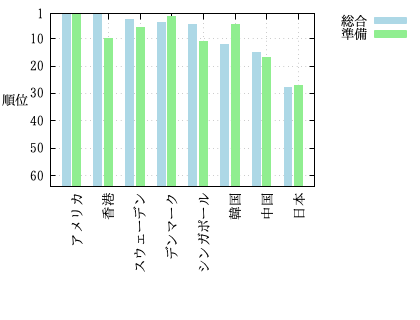
\includegraphics[width=0.7\linewidth]{fig51.png}
\caption{デジタル競争力ランキング}\label{fig:保有率}
\end{figure}% 節見出し: \section{}
% を使う

\section{ブロードバンドの整備状況}

OECDによるブロードバンド回線の普及に関する調査\cite{oecd}によると、表\ref{tbl:利用状況}に示すように、日本における 100人あたりのモバイルブロードバンドの加入者数は190.5で、第1位になっている。2位はエストニア
で、3位米国と続く。

\begin{table}[htbp]
    \centering
    \caption{モバイルブロードバンドの加入者数(100人あたり)}
    \label{tbl:利用状況}

    \begin{tabular}{|c|l|r|}
        \hline
        順位 & 国名 & 加入者数 \\
        \hline
        1位 & 日本 & 190.5\\
        \hline
        2位 & エストニア & 179.9\\
        \hline
        3位 & 米国 & 169.0\\
        \hline
        4位 & フィンランド & 157.0\\
        \hline
        5位 & デンマーク & 141.7\\
        \hline
        6位 & ラトビア & 141.6\\
        \hline 
        7位 & イスラエル & 139.9\\
        \hline
        8位 & オランダ & 133.7\\
        \hline
        9位 & ポーランド & 131.3\\
        \hline
        10位 & スウェーデン & 127.2\\
        \hline
    \end{tabular}
\end{table}

\section{考察}

\begin{itemize}
    \item 日本はモバイルブロードバンドの普及率が世界で1位だが、デジタル競争力では28位と低くインフラをうまく活かしきれていない現状があると感じる。
    \item デジタル競争力の順位が低いことから、今後、競争力を高めていくには、IT教育が急務であると考えられる。
\end{itemize}

% 節見出し: \section{}
% を使う

% \section{考察}
% \begin{itemize}
%     \item 箇条書き
%     \item 箇条書き
% \end{enumerate}

%  参考文献の参照: \cite{}
%  図番号の参照: \ref{}
% を使う
% 文献データベースのキーワードは oecd と imd
% になっている.

% 図の挿入
% \includegraphics{}
% を
% \begin{figure}[htbp]
% \end{figure}
% で囲み
% \caption{}
% で図のタイトルを入れる.
% \label{}
% を使って図番号が参照できるようにする
% また,
% \centering
% で図が中央に来るようにする

% ーーー
% 節見出し(2)

% 本文(2)

% 表の挿入
% \begin{tabular}
% \end{tabular}    
% による表の記述を 
% \begin{table}[htbp]
% \end{table}
% で囲み
% \caption{}
% で表のタイトルを入れる.
% \label{}
% を使って表番号が参照できるようにする
% また,
% \centering
% で表が中央に来るようにする

% ーーー
% 見出し(3)
% 考察
%
% \begin{itemize}
% \end{itemize}
% を使って箇条書きで記述する

% ここに参考文献が入る
%
\bibliographystyle{junsrt}
\bibliography{exercise.bib}

\end{document}